%==============================================================================
%  Paper 3 —— 中文版
%  动力学冻结而非平衡：闪锌矿中的铟纳米包裹体何以存续
%
%  余贺、陈汝清、卢焕章
%
%  编译:  xelatex paper3_zh.tex   (连续运行两次以解析交叉引用)
%  字体:  Noto Serif CJK SC / Noto Sans CJK SC
%
%  说明: 本文为英文正式稿 paper3.pdf 的中文译本，内容完全对应。图件坐标轴
%        标注保持英文原样，图题已译出。术语沿用系列前两篇中文版的译法。
%==============================================================================
\documentclass[11pt,a4paper]{ctexart}

\usepackage[margin=2.5cm]{geometry}
\usepackage{amsmath,amssymb}
\usepackage{booktabs}
\usepackage{graphicx}
\usepackage{authblk}
\usepackage{caption}
\usepackage[round,authoryear]{natbib}
\usepackage[hidelinks]{hyperref}
\usepackage{url}

\setCJKmainfont{Noto Serif CJK SC}
\setCJKsansfont{Noto Sans CJK SC}

\graphicspath{{../figures/}{figures/}{./}}
\captionsetup{font=small,labelfont=bf}
\setlength{\parskip}{2pt}
\linespread{1.15}

\renewcommand\Authsep{，}
\renewcommand\Authand{，}
\renewcommand\Authands{，}
\renewcommand\Affilfont{\small}
\renewcommand{\refname}{参考文献}

\newcommand{\dQ}{\Delta Q}
\newcommand{\JCuIn}{J_{\mathrm{Cu\text{-}In}}}
\newcommand{\Jlike}{J_{\mathrm{like}}}
\newcommand{\Tf}{T_{\mathrm{f}}}

\title{\bfseries 动力学冻结而非平衡：\\
闪锌矿中的铟纳米包裹体何以存续}

\author[1]{余贺}
\author[2]{陈汝清\thanks{通讯作者。}}
\author[3]{卢焕章}
\affil[1]{贺州学院 地质实验室，广西 贺州 542899，中国}
\affil[2]{GUT Geoservice Inc.，加拿大 魁北克省 蒙特利尔}
\affil[3]{魁北克大学希库蒂米分校 应用科学系与矿产资源研究中心，加拿大 魁北克省}
\date{}

\begin{document}
\maketitle

\noindent\small
\textit{电子邮箱：} \texttt{yuhe@hzxy.edu.cn}（余贺），
\texttt{ruqing@hotmail.com}（陈汝清），
\texttt{hzlu@uqac.uquebec.ca}（卢焕章）。
\normalsize

\noindent\small
\textbf{版本 2.0。} 本版报告了版本 1 所提出但尚未执行的一项检验的结果。
第~\ref{sec:crosscheck} 节曾指出粗化指数的四项测定跨越三倍，而
第~\ref{sec:discussion} 节提出这或许反映了一种交叉过渡：自原子尺度的界面限制
粗化随畴长大而转向扩散限制粗化，并指出该提议可在单次模拟内检验。此后我们在
四种界面宽度下作了相场运行，该假说\emph{未}获支持：以界面宽度重标后曲线并不
塌缩，且指数上升而非下降。指数真正跟随的是每次运行推进的程度，其与步数对数的
相关系数为 0.99，这指向一个自下方被趋近的共同渐近值。版本 1 的其余结论均未
改变；第~\ref{sec:geospeedometer} 节的分歧回到未成对配对的端元数据这一余下
解释。详见第~\ref{sec:discussion} 节。
\normalsize

\begin{abstract}
\noindent
铟在闪锌矿中的平衡态是单一凝聚畴：本系列前一篇已在 0.10 至 2.00~at.\% 的每一个
成分下确立了这一点；本文进一步表明，将一个畴一分为二的代价为 300 至
1800~$k_BT$，其依据是界面能的闭式解
$\gamma = \lambda/3 - J_{\rm Cu\text{-}In}/3 - J_{\rm like}/6$，其中体相项精确
抵消。然而天然闪锌矿仍普遍携带离散的纳米级与微米级包裹体群。所观测到的构型
比自由能所选定的状态高出数百 $k_BT$。

我们论证这是动力学冻结而非热力学的失效，并且该论证把一个空间问题——包裹体
有多大——转化为一个时间问题。粗化受溶质输运限制，而输运是热激活的，故其时标
随降温呈指数增长；冷却时标却仅按 $T^2$ 下降。两者必然相交，且只交一次。在
交点以下微结构停止演化，存续下来的不是平衡态，而是输运停止时体系恰好所处的
构型。

冻结条件受到强烈缓冲：进入其中的每一个量——包括本工作无法确定的扩散前因子
——都出现在一个对数之内，故其中任何一个错一个数量级，冻结温度的移动都不足
四分之一。由此冻结畴尺寸随冷却速率呈幂律 $R_{\rm f} \propto |\dot{T}|^{-n}$，
其中承载物理的是指数而非前因子。

支撑这一论证的是两项计算，其角色不可互换。体相自由能由热力学积分测得而非
假设，因为正则溶液形式在本体系中根本没有驱动力——在均匀混合下异价与同价贡献
精确相消；梯度能系数随后由 $\gamma$ 确定。在此基础上的相场计算重现了从均匀
固溶经旋节分解至粗化与冻结的完整序列，给出 $n = 0.259$；但它无法给出绝对
长度，因为界面必须被数值展宽才能被任何求解器分辨。而界面保持其物理宽度（一个
键宽）的直接格点粗化，给出一至二纳米的畴与 $n = 0.150$。

与冷却速率跨越八个数量级的矿床类型（自淬火的海底体系至盆地卤水）相对照，
模型重现了所观测到的包裹体尺寸排序，但隐含的指数接近 $0.45$，高于任一模拟值。
我们报告这一分歧而非其吻合。一个候选解释——自原子尺度的界面限制粗化向畴长大后
的扩散限制粗化过渡——此后已由四种界面宽度下的相场运行加以检验，未获支持：以界面
宽度重标后曲线并不塌缩，且指数上升而非下降。在该问题
解决之前，反演只支持对矿床按冷却速率排序，而不支持标定某一速率。

无论如何，有两项推论成立。平滑的 LA-ICP-MS 深度剖面是快速冷却的证据而非固溶体
的证据，因为铟已经聚集，只是低于剥蚀体积的分辨能力。而铟的赋存状态、进而其
冶金回收行为，应当在不同矿床类型之间沿一条可由热历史预先判断的轴系统地变化。
\end{abstract}

%==============================================================================
\section{引言}
\label{sec:intro}

\subsection{一个结果与一处矛盾}

本系列前一篇通过对构型哈密顿量的并行回火采样确立：铟在闪锌矿中的平衡态是凝聚
的 \citep{yu2026b}；该哈密顿量的电荷补偿系数由 ZnS 的介电常数确定而非拟合。
在所考察的每一个成分下——自 0.10 至 2.00~at.\%——溶质都聚集为\emph{单一}畴：
单体占比全程为零，而最稀点处随机固溶体的预期为 98\%；且该结果由夹逼而非由
收敛确立，故它不依赖于让一个在成矿温度下无法平衡的采样器达到平衡。

本文第~\ref{sec:gamma} 节量化了该状态为何是单一而非仅仅凝聚。界面能拥有闭式解
$\gamma = \lambda/3 - \JCuIn/3 - \Jlike/6$，其中体相项精确抵消；在所考察的
尺寸范围内，将一个畴一分为二的代价为 300 至 1800~$k_BT$。体相构型热力学以
巨大的裕度反对彼此分离的畴群。

天然闪锌矿却经常携带一群。高分辨显微学在 LA-ICP-MS 深度剖面完全平滑的样品中
分辨出数十纳米尺度的含铟不均匀性 \citep{cook2009,frenzel2016}；硫铟铜矿亦有
作为自闪锌矿出溶的离散微米级颗粒的报道 \citep{moura2007}。二者都不是单一畴。
这一矛盾是尖锐的，而且是定量的而非解释性的：所观测的构型比自由能所选定的
状态高出数百 $k_BT$。

\subsection{该矛盾只是表观的}

前述结果中没有任何一处断言闪锌矿颗粒\emph{达到}其平衡构型。平衡热力学识别的是
体系在时间不受限制时会到达的状态；它对时间是否够用不置一词。矿体会冷却，而
随着冷却，本可把微结构带向平衡的溶质输运呈指数变慢，冷却本身却以地质条件设定
的速率进行。在某个温度以下，后者超过前者，微结构随之停止演化。存续下来供人
观测的不是平衡态，而是输运停止时体系恰好占据的那个状态。

这就是动力学冻结，而本文的主张是它足以完整解释上述差异。天然闪锌矿的多畴结构
既非另一种平衡态，亦非对 \citet{yu2026b} 之热力学的反证；它们就是那套热力学
被打断的结果。

该主张有一个可检验的推论，这也是它值得论证而非仅仅断言的原因。若包裹体是被
冻结的粗化产物，则其尺寸记录了粗化在停止之前拥有多少时间，因而也记录了岩石
冷却得有多快。空间问题——包裹体有多大——由此成为一个时间问题。

\subsection{完成该论证需要什么}

把一个空间问题转化为时间问题需要三样东西，本文依次提供。

其一，格点模型的热力学必须被带入一个可以追踪粗化的连续介质描述。
第~\ref{sec:bridge} 节在不引入任何可调参数的前提下完成这一步：体相自由能由
热力学积分测得而非假设，因为正则溶液形式在本体系中\emph{没有}驱动力——在均匀
混合下异价与同价贡献精确相消；而梯度能系数由界面能确定，后者由
第~\ref{sec:gamma} 节以闭式给出并经显式构造验证。

其二，粗化与冷却之间的竞争必须被明确写出。第~\ref{sec:timescales} 节表明：
降温时粗化时标呈指数增长而冷却时标仅按 $T^2$ 下降，故二者必然相交且只交一次；
交点温度对进入其中的每一个量——包括本工作无法确定的扩散前因子——都受到对数
缓冲；由此冻结畴尺寸随冷却速率呈幂律。

其三，该预言必须与观测对质。第~\ref{sec:geospeedometer} 节把幂律与冷却速率
相差八个数量级、包裹体结构相差四个数量级的矿床类型相对照。排序被重现了。
量级没有，而我们报告这一分歧及其可能来源，而非其吻合。

\subsection{两种方法，各自的用途}

本文使用两项计算，其角色不可互换；完整的分工见第~\ref{sec:kappacaveat} 节，
此处提及是因为它决定了后续每一幅图应当如何解读。

相场计算提供\emph{路径与拓扑}：体系经历哪些形貌、粗化是完成还是冻结，以及
结果如何依赖于冷却速率与迁移率之比。它\emph{无法}提供绝对长度，因为
Cahn--Hilliard 界面必须被数值展宽才能被任何求解器分辨，故那些图中的畴尺寸是
由网格设定而非预言的。

直接格点粗化模拟提供\emph{绝对尺度}，界面保持其一个键宽的物理宽度，任何环节
都不作展宽。它所能触及的时间与畴数远少于前者，但它的纳米就是纳米。

在两者都能计算的量上——粗化指数——我们作了比较，而
第~\ref{sec:crosscheck} 节报告二者相差 70\%。该分歧及其所动摇与未动摇的部分，
在那里处理而非推迟。

%==============================================================================
\section{从格点到连续介质}
\label{sec:bridge}

守恒序参量 $c(\mathbf{r}, t)$ 的 Cahn--Hilliard 方程 \citep{cahn1958}——此处
$c$ 为阳离子亚晶格上的总溶质分数 $x_{\rm Cu} + x_{\rm In}$——为
\begin{equation}
\frac{\partial c}{\partial t}
  = \nabla \cdot \left[ M(T)\, \nabla \frac{\delta F}{\delta c} \right],
\qquad
F[c] = \int \left[ f(c) + \tfrac{1}{2}\kappa \left|\nabla c\right|^2 \right] \mathrm{d}V .
\label{eq:ch}
\end{equation}
须提供三个量：体相自由能密度 $f(c)$、梯度能系数 $\kappa$、迁移率 $M(T)$。
本节在不引入可调参数的前提下由格点模型获得前两者，并说明关于第三者已知与
未知的部分。

\subsection{为何 $f(c)$ 不能假设}
\label{sec:whynotregular}

通常的做法是假定一个正则溶液或双阱形式的 $f(c)$ 并拟合其系数。这在此处不可行，
而障碍是本哈密顿量所特有的，而非精度问题。

在 $x_{\rm Cu} = x_{\rm In} = c/2$ 的均匀混合下，电荷补偿能的构型部分平均为
\begin{equation}
\Big\langle \sum_{\langle ij \rangle} \delta q_i \delta q_j \Big\rangle_{\rm rand}
= \frac{Nz}{2}\left[ 2\left(\frac{c}{2}\right)^2(-1)
                   + \left(\frac{c}{2}\right)^2(+1)
                   + \left(\frac{c}{2}\right)^2(+1) \right] = 0,
\label{eq:mfzero}
\end{equation}
因为携带 $\delta q_i \delta q_j = -1$ 的异价 Cu--In 接触，与携带 $+1$ 的同价
Cu--Cu 及 In--In 接触精确相消。因此建立在均匀混合之上的平均场自由能在任何成分
下都\emph{完全没有驱动力}。本体系的全部热力学都住在平均场所丢弃的关联之中；
用自由能的语言来说，这与 \citet{yu2026b} 中"平衡态是凝聚的而随机固溶体不是"
这一观察是同一句话。

其后果是：正则溶液形式的 $f(c)$ 并非对本体系的一个近似，而是对另一个体系的
描述。$f(c)$ 必须实测。

\subsection{以热力学积分测定 $f(c)$}
\label{sec:fofc}

我们通过对耦合强度积分得到 $f(c)$。引入标度参数 $a \in [0,1]$ 并令
$H(a) = aH$，则完全耦合体系的自由能为
\begin{equation}
F(1) = F(0) + \int_0^1 \langle H \rangle_a \, \mathrm{d}a,
\label{eq:ti}
\end{equation}
其中 $F(0)$ 为理想溶液自由能，解析地等于每格位
$-k_BT \sum_\alpha x_\alpha \ln x_\alpha$，而 $\langle H \rangle_a$ 是完整
哈密顿量在由 $H(a)$ 生成的系综中的期望。该恒等式是精确的；唯一的误差来自
$\langle H \rangle_a$ 的采样误差与求积误差，二者都可控。

标度\emph{整个}哈密顿量而非其中一项是要紧的。沿着只标度 $E_c$ 的路径积分会给出
那条路径上的自由能差，那是另一个量；式~\eqref{eq:ti} 的恒等式要求 $a$ 整体地
乘在 $H$ 上。

表~\ref{tab:fofc} 给出 573~K 下的结果，在 $L = 12$ 盒子（$N = 6912$ 个阳离子
格位）中计算，$a$ 方向取九个 Gauss--Legendre 节点，每个节点上作块平均采样。

\begin{table}[htbp]
\centering
\caption{573~K 下每阳离子格位的体相自由能，由热力学积分得到。$f_{\rm ideal}$
为理想溶液项，积分列为 $\int_0^1 \langle H\rangle_a\,\mathrm{d}a$。不确定度
由各求积节点上块平均的采样误差传播而来。}
\label{tab:fofc}
\small
\begin{tabular}{rrrrr}
\toprule
$c$ & $f_{\rm ideal}$ (eV) & 积分 (eV) & $f(c)$ (eV) & $\pm$ \\
\midrule
0.005 & $-0.00173$ & $0.00232$ & $+0.00059$ & 0.00002 \\
0.010 & $-0.00311$ & $0.00399$ & $+0.00089$ & 0.00003 \\
0.020 & $-0.00553$ & $0.00653$ & $+0.00101$ & 0.00004 \\
0.040 & $-0.00966$ & $0.01049$ & $+0.00083$ & 0.00024 \\
0.080 & $-0.01650$ & $0.01436$ & $-0.00214$ & 0.00038 \\
0.120 & $-0.02222$ & $0.01965$ & $-0.00258$ & 0.00045 \\
0.160 & $-0.02719$ & $0.02313$ & $-0.00405$ & 0.00041 \\
0.200 & $-0.03155$ & $0.02642$ & $-0.00513$ & 0.00052 \\
\bottomrule
\end{tabular}
\end{table}

\subsection{不稳定性，以及如何稳健地诊断它}
\label{sec:spinodal}

Cahn--Hilliard 不稳定性要求 $f''(c) < 0$。然而从八个测点中提取二阶导数是一个
病态运算，我们以相应的谨慎报告它。

拟合多项式再求两次导，所得答案依赖于所选阶数：在 $c = 0.20$ 处，三次、四次与
五次拟合分别返回 $f'' = +0.62$、$-2.90$ 与 $+7.23$~eV。这不是同一个数的三个
估计，而是一个欠定拟合的振荡。对原始点作有限差分表现稍好，但在浓端相邻区间之间
仍会变号。

具有物理意义的检验不是局域曲率，而是共切线构造——它追问成分为 $c$ 的均匀态是否
比另外两个成分的混合物具有更高的自由能，且完全不需要求导。取所测范围两端之间
的弦，超出量 $f(c) - f_{\rm chord}(c)$ 为
\begin{center}
\small
\begin{tabular}{rrrrrrrr}
\toprule
$c$ & 0.005 & 0.010 & 0.020 & 0.040 & 0.080 & 0.120 & 0.160 \\
\midrule
$f - f_{\rm chord}$ ($10^{-5}$ eV) & $0$ & $+44$ & $+86$ & $+126$ & $-53$ & $+21$ & $-9$ \\
\bottomrule
\end{tabular}
\end{center}
0.010 至 0.040 的稀成分高出弦达其采样不确定度的三至五倍，因而对相分离不稳定。
浓成分在不确定度范围内位于弦上或弦下。

由此有两点。其一，不稳定性位于稀成分区间，而那正是 \citet{yu2026b} 发现完全
凝聚之处，也是天然闪锌矿所处之处：自由能测量与直接模拟由两条独立途径彼此吻合。
其二，分辨相界本身所需的成分间距与误差棒均超出本采样所能提供者；我们把 $f(c)$
用作式~\eqref{eq:ch} 中的驱动力，而不声称已定位双节线。

两类不稳定性的区别对下文是要紧的。位于共切线之上但曲率为正的成分是\emph{亚稳}
的：它只能经由成核、越过势垒而分离。曲率为负者则彻底\emph{不稳定}，会自发分离，
且在长于某个临界值的每一个波长上都如此——即旋节分解。第~\ref{sec:pf} 节的模拟
在后一种情形下进行，以便在不引入成核速率这一另行不确定的物理的前提下展示路径。
天然闪锌矿究竟以旋节方式还是以成核方式分解，取决于其成分相对于一条本工作未能
分辨的界线的位置；而本文所关心的冻结物理在两种情形下相同，因为它取决于输运的
停止，而非分解如何开始。

\subsection{梯度系数由界面能确定}
\label{sec:kappa}

对于处于平衡的平面界面，Cahn--Hilliard 泛函给出界面能为
\begin{equation}
\gamma = \int_{c_\alpha}^{c_\beta} \sqrt{2\kappa\, \Delta f(c)}\ \mathrm{d}c,
\qquad
\Delta f(c) = f(c) - f_{\rm tangent}(c),
\label{eq:gammakappa}
\end{equation}
其中 $f_{\rm tangent}$ 为共存成分 $c_\alpha$ 与 $c_\beta$ 之间的共切线。由于
$\gamma$ 已由格点模型以闭式给出（第~\ref{sec:gamma} 节）而 $f(c)$ 现已测得，
式~\eqref{eq:gammakappa} 即确定 $\kappa$。它不是一个拟合参数。

\subsection{这套桥接给不了什么：绝对长度尺度}
\label{sec:kappacaveat}

本小节陈述一项限制，它决定了第~\ref{sec:pf} 节的相场结果应当如何解读；我们在
给出其中任何一项结果\emph{之前}先行陈述。

Cahn--Hilliard 方程的特征长度为 $\ell = \sqrt{\kappa / |f''|}$，它设定界面宽度。
当 $\kappa$ 由式~\eqref{eq:gammakappa} 从一个原子尺度的量——格点模型的界面只有
一个键宽——确定时，物理的 $\ell$ 即为晶格参数量级。没有任何有限差分或谱方法
求解器能表示如此之薄的界面：数值稳定性要求界面跨越四至六个网格点，故任何实际
计算都必须要么采用远小于晶格参数的网格间距（那毫无意义），要么膨胀 $\kappa$
使界面在可用网格上铺开。

本文报道的每一次相场计算都采取后一条路，正如任何针对原子级锐界面的相场计算都
必须如此。其后果不可避免，且不容遮掩：\emph{相场模拟中出现的畴尺寸是由网格间距
设定的，而非由物理预言的}。若读者追问为何所模拟的包裹体恰好是纳米尺度，诚实的
回答是网格就是那样选的。

因此我们明确划分两种方法的分工。

\begin{itemize}\itemsep2pt
\item \textbf{相场模型提供路径与拓扑}：体系所经历的形貌序列、粗化是完成还是
冻结，以及该结果如何依赖于冷却速率与迁移率之比。这些都是无量纲陈述，不受
$\kappa$ 膨胀的影响，因为膨胀 $\kappa$ 会同时重标长度与时间。
\item \textbf{格点模型提供绝对尺度}：以原子数与纳米计的畴尺寸，由直接粗化模拟
（第~\ref{sec:latticecoarsen} 节）得到，其中界面就是它物理上的样子，不发生任何
膨胀。
\end{itemize}

二者在都能计算的量上——即粗化指数——于第~\ref{sec:crosscheck} 节交叉验证。

\subsection{迁移率}
\label{sec:mobility}

迁移率是本工作唯一无法从格点模型获得的输入，因为蒙特卡洛扫程不是物理时间。
因此我们以无量纲迁移率建立框架，并另行说明赋予其绝对单位需要什么。

替代型亚晶格中的溶质输运是热激活的，故
\begin{equation}
M(T) = \frac{D(T)\, \Omega}{k_B T}, \qquad
D(T) = D_0 \exp\!\left(-\frac{E_a}{k_B T}\right),
\label{eq:arrhenius}
\end{equation}
其中 $\Omega$ 为每阳离子格位的体积。激活能 $E_a$ 有一个来自模型自身的下界：
把一个溶质移出畴需要打断其异价键，每条代价 $2\lambda \approx 0.6$~eV，故对表面
溶质有 $E_a \gtrsim 2\lambda$，对内部溶质则为其数倍。这是界而非测定：真实的
$E_a$ 还包含底层扩散机制（无论是空位介导还是间隙介导）的迁移势垒，而构型模型
不表示那一部分。

由此有两类结论，我们全文予以标注。

\emph{仅需阿伦尼乌斯形式的结论。} 第~\ref{sec:timescales} 节所展开的粗化与
冷却之竞争、冻结温度的存在性，以及最终畴尺寸对冷却速率的标度，全部由
式~\eqref{eq:arrhenius} 的\emph{形式}连同 $E_a > 0$ 推出。它们以约化变量表达，
不需要 $D_0$ 的绝对值。

\emph{需要 $D_0$ 与 $E_a$ 的结论。} 把冻结温度放到绝对标度上，以及把观测到的
畴尺寸分布换算为以开尔文每年计的冷却速率，都需要 Cu 或 In 在闪锌矿中扩散数据的
实测值。有此类数据可用之处我们予以使用并加以标明；无可用者则以相对标定报告，
即畴尺寸之比映射到冷却速率之比而二者皆非绝对。我们认为相对标定是更稳妥的主张，
也是本工作所确立的那一个。


%==============================================================================
\section{界面能与分裂势垒}
\label{sec:gamma}

溶质畴与 ZnS 基质之间的界面能在此处两次被用到：其一，经由
式~\eqref{eq:gammakappa} 确定 $\kappa$；其二，设定本文所要解释其存续的多畴构型
所需付出的热力学代价。它可以以闭式给出。

\subsection{闭式解}
\label{sec:gammaclosed}

考虑一个含 $n$ 个溶质（Cu 与 In 各半）的畴，并令 $A$ 为溶质--Zn 第一近邻键数，
这是以晶格自身的自然单位度量的界面。溶质提供 $12n$ 个键端，其中 $A$ 个伸向
基质，故溶质--溶质键数为 $N_{ss} = (12n - A)/2$。在理想的 2Cu+2In 序中，每个
阳离子有八个异价近邻与四个同价近邻，故指向溶质的键端中有三分之二是异价的：
\begin{equation}
N_{\rm CuIn} = \tfrac{1}{3}(12n - A) = 4n - \tfrac{A}{3},
\qquad
N_{\rm like} = 2n - \tfrac{A}{6}.
\label{eq:bondcounts}
\end{equation}
代入电荷补偿能的精确对形式 \citep{yu2026}，
\begin{equation}
E_c = 4\lambda \sum_i \delta q_i^{\,2}
    + 2\lambda \sum_{\langle ij \rangle} \delta q_i \delta q_j
    = 16\lambda n - \lambda A - 4\lambda\left(4n - \frac{A}{3}\right)
    = \frac{\lambda}{3} A .
\label{eq:Ecgamma}
\end{equation}
体相项精确抵消，只留下一个严格正比于界面面积的能量。加上化学项即得
\begin{equation}
\boxed{\;
\gamma = \frac{\lambda}{3} - \frac{\JCuIn}{3} - \frac{\Jlike}{6}
\;}
\label{eq:gamma}
\end{equation}
（每条溶质--Zn 键），相应的体相系数为
\begin{equation}
e_{\rm bulk} = 4\JCuIn + 2\Jlike
             + \tfrac{1}{2}\left(E_s^{\rm Cu} + E_s^{\rm In}\right)
\label{eq:ebulk}
\end{equation}
（每个溶质）。其中 Eshelby 项取两个物种的\emph{平均}而非单取铟的值，因为
$e_{\rm bulk}$ 是按每溶质原子表达的，而化学计量畴中两个物种数目相等。铜对它
毫无贡献：四配位下 $r_{\mathrm{Cu^+}} = r_{\mathrm{Zn^{2+}}} = 0.60$~\AA{}，
其失配恒为零，故 $E_s^{\rm Cu} = 0$ 而 $E_s^{\rm In} = 0.033$~eV。在
\citet{yu2026} 的参数下，$\gamma = 0.125$~eV/键，$e_{\rm bulk} = -0.2835$~eV/
溶质。

式~\eqref{eq:gamma} 有两点值得强调。它不含任何拟合量：$\lambda$ 由 ZnS 的
介电常数确定，而 $J$ 项显式出现，故该表达式在任何未来的第一性原理测定给出后
可立即更新，无需重跑任何模拟。此外，式~\eqref{eq:Ecgamma} 中的抵消是精确的而非
渐近的，故该结果对任意尺寸的畴成立，而不仅对大畴成立。

\subsection{显式构造的验证}
\label{sec:gammaverify}

在 $L = 24$ 盒子（$N = 55{,}296$ 个阳离子格位）中显式构建了 64 至 3072 个溶质
的七种尺寸的畴并精确求值，随后仅以溶质--溶质交换在 20~K 下弛豫。如此限制移动集
可让界面在化学上重构，同时使畴的外形（因而 $A$）严格保持不变；这把界面项与
溶解物理分离开来。

\begin{table}[htbp]
\centering
\caption{闭式解与显式构造给出的界面系数与体相系数，$L = 24$，自 64 至 3072 个
溶质的七种畴尺寸。}
\label{tab:gamma}
\small
\begin{tabular}{lrr}
\toprule
& $e_{\rm bulk}$（eV/溶质） & $\gamma$（eV/键） \\
\midrule
闭式解，式~\eqref{eq:gamma} & $-0.2835$ & $0.1250$ \\
构造所得 & $-0.2394$ & $0.1557$ \\
弛豫之后 & $-0.2802$ & $0.1281$ \\
\bottomrule
\end{tabular}
\end{table}

弛豫后的构造与闭式解在 $e_{\rm bulk}$ 上吻合到 1.2\%、在 $\gamma$ 上吻合到
2.5\%，而这一吻合值得的不只是一句"数值自洽"。式~\eqref{eq:gamma} 是一个连续介质
陈述：它断言两相构型的过剩能量严格正比于界面\emph{面积}，且其系数与尺寸和形状
无关。同一个系数能够重现含 64 个溶质的畴——那是约一纳米大小、多数原子位于表面的
对象——这表明整个连续介质处理所依赖的面积缩放律在本体系中并未在纳米尺度失效。
其原因在式~\eqref{eq:Ecgamma} 中一目了然：体相项的抵消是精确的而非渐近的，故
并未援引任何大畴极限。这正是使用 Cahn--Hilliard 泛函描述天然闪锌矿实际所含
尺寸的包裹体的许可证。

未弛豫构造之所以偏高，是因为层状序规则在表面无法精确满足：所构造的畴比理想异价
键数低 1.5\% 至 5.4\%，而该缺额随尺寸增大而减小（表面占比下降），弛豫恢复了其中
大部分。两项拟合的残差在 450~eV 的能量跨度上为 5.1~eV 均方根；加入一个
$n^{1/3}$ 的棱边项仅将其降至 4.92~eV，故在此范围内两项描述已经足够。

\subsection{分裂一个畴的代价}
\label{sec:splitting}

将一个畴一分为二所需的能量为
$\Delta E = \gamma\left[2A(n/2) - A(n)\right]$，以弛豫后的 $\gamma$ 与实测面积
求值：

\begin{center}
\small
\begin{tabular}{rrrrr}
\toprule
$n$ & $A(n)$ & $2A(n/2)$ & $\Delta E$ (eV) & 573~K 下的 $\Delta E / k_BT$ \\
\midrule
128  & 414  & 528  & 14.6 & 296 \\
256  & 642  & 828  & 23.8 & 483 \\
512  & 1040 & 1284 & 31.3 & 633 \\
1024 & 1640 & 2080 & 56.4 & 1141 \\
2048 & 2598 & 3280 & 87.4 & 1769 \\
\bottomrule
\end{tabular}
\end{center}

每一个值都为正——分裂一个畴必然增加界面面积，故必须如此——且每一个值相对热能都
极其巨大。这就是本文所处理的问题的定量形式：体相构型热力学以数百 $k_BT$ 反对
彼此分离的畴群，而天然闪锌矿所展示的恰恰常常就是这样的畴群。其解答不可能是
热力学的。

\subsection{两个不应采用的采样估计}
\label{sec:gammafailed}

在闭式解之前有两次有限温测定 $\gamma$ 的尝试，均告失败。此处记录它们，因为其
失效方式诊断出一个普遍的困难：$\gamma$ 是大数之间的小差值，而采样所得的构型
同时携带能量误差与形状噪声。

第一次在 573~K 下等温弛豫各畴，那里接受率约为 $10^{-5}$，结果把 $n = 1280$ 的
畴停在 $-145$~eV，而独立已知的平衡界限为 $-298$~eV。第二次改用并行回火，达到
$-228$~eV——有所改善，但仍短缺 24\%——并且在 $n = 1280$ 处返回了一个三团簇构型，
故所测面积属于三个畴而非一个。其诊断性失效毫不含糊：$n = 640$ 处拟合出的分裂
代价为\emph{负值}，而这不可能。

闭式解通过完全不采样而规避了这两项困难。第~\ref{sec:gammaverify} 节对它的验证
使用构造与零温弛豫，其中畴的外形是被施加的而非被推断的。

%==============================================================================
\section{两个相互竞争的时标}
\label{sec:timescales}

第~\ref{sec:bridge} 与 \ref{sec:gamma} 节确立：两相构型每条畴界都携带数百
$k_BT$ 量级的界面代价，故彼此分离的畴群在热力学上被强烈地不利。
\citet{yu2026b} 表明平衡态是单一凝聚畴。天然闪锌矿却经常携带许多。本节说明
何以如此，且其形式不需要任何模拟。

\subsection{两个速率}

粗化经由输运进行：物质必须离开较小的畴、抵达较大的畴，穿越一个每走一步都需要
打断异价键的基质。对半径为 $R$ 的畴的扩散限制粗化，
Lifshitz--Slyozov--Wagner 结果 \citep{lifshitz1961} 给出
$R^3 - R_0^3 \propto D t$，故使一个畴显著长大所需的时间为
\begin{equation}
\tau_{\rm coarsen}(T) \;\sim\; \frac{R^3\, k_B T}{\gamma\, D(T)\, \Omega},
\qquad
D(T) = D_0 \exp\!\left(-\frac{E_a}{k_B T}\right),
\label{eq:taucoarsen}
\end{equation}
其中 $\Omega$ 为每阳离子格位的体积。界面能出现在分母中，是因为它就是驱动力：
更大的 $\gamma$ 使粗化更快而非更慢。

冷却提供与之竞争的速率。要紧的不是绝对的温降，而是迁移率发生显著变化所经历的
时间，因为那正是体系或粗化或不粗化的时间窗口。对阿伦尼乌斯形式求导，迁移率在
温度区间 $k_BT^2/E_a$ 内下降 $e$ 倍，故
\begin{equation}
\tau_{\rm cool}(T) \;\sim\; \frac{k_B T^2}{E_a\, \lvert \dot{T} \rvert}.
\label{eq:taucool}
\end{equation}

本质的不对称性至此显现。随着温度下降，$\tau_{\rm coarsen}$ 经由阿伦尼乌斯因子
呈\emph{指数}增长，而 $\tau_{\rm cool}$ 仅按 $T^2$ 下降。无论二者在高温下如何
排序，它们都必然相交，且只交一次。

\subsection{冻结温度}

令 $\tau_{\rm coarsen}(\Tf) = \tau_{\rm cool}(\Tf)$ 并取对数，得冻结条件
\begin{equation}
\frac{E_a}{k_B \Tf}
 = \ln\!\left[ \frac{\gamma\, D_0\, \Omega\, \Tf}
                    {R^3\, E_a\, \lvert \dot{T} \rvert} \right].
\label{eq:arrest}
\end{equation}
在 $\Tf$ 以下微结构被冻结：粗化仍会降低自由能，而且降幅巨大，但已不再有时间。
存续下来供人观测的构型，就是输运停止时体系恰好所处的那一个。

式~\eqref{eq:arrest} 对 $\Tf$ 是超越的，但它的结构比它的解更有信息量。左端是
一个大数——取 $E_a \gtrsim 2\lambda \approx 0.6$~eV 且 $\Tf$ 处于成矿温度范围
时，$E_a/k_B\Tf$ 介于 9 与 17 之间——而右端是一个对数。对数不可能变化得快，
因此 $\Tf$ 对其中的一切都受到强烈缓冲。隐式求导，令 $X = E_a/k_B\Tf$，
\begin{equation}
\frac{\mathrm{d}\Tf}{\Tf} = -\frac{\mathrm{d}\ln \lvert\dot{T}\rvert}{X - 1}.
\label{eq:tfsens}
\end{equation}
冷却速率提高十倍，使 $\Tf$ 在 400~K 处上升 14\%、573~K 处 21\%、800~K 处 30\%。
因此冻结温度是冷却历史的弱函数；它对 $D_0$、$\gamma$ 与 $R$ 的依赖亦然，因为
这些量都只以对数形式进入。

这是一项有用的稳健性而非限制。它意味着冻结的存在及其大致位置，并不依赖于本
工作无法确定的那些量：$D_0$ 有一个数量级的不确定度，只会使 $\Tf$ 移动不足
四分之一。

\subsection{被冻结下来的是什么}

冻结时的畴尺寸，可由计算两个时标相交时粗化已经推进到何处而得到。将
$\tau_{\rm cool}(\Tf)$ 代入 Lifshitz--Slyozov 增长律，
\begin{equation}
R_{\rm f}^3 \;\sim\; \frac{\gamma\, D(\Tf)\, \Omega}{k_B \Tf}\,
                     \tau_{\rm cool}(\Tf)
             \;\sim\; \frac{\gamma\, D_0\, \Omega}{E_a\, \lvert\dot{T}\rvert}
                      \, \Tf \exp\!\left(-\frac{E_a}{k_B \Tf}\right).
\label{eq:Rf}
\end{equation}
由于 $\Tf$ 本身仅随 $\lvert\dot{T}\rvert$ 作对数变化，显式因子占主导，因而
\begin{equation}
\boxed{\;R_{\rm f} \;\propto\; \lvert\dot{T}\rvert^{-n}, \qquad n \to 1/3 \;}
\label{eq:scaling}
\end{equation}
——此为忽略 $\Tf$ 漂移时的极限；一旦不忽略，$n$ 会低于 $1/3$，因为更快的冷却
在更高的温度处冻结，而那里迁移率更大，从而部分抵消。第~\ref{sec:pf} 节的相场
模拟给出 $n = 0.259$，与一个被上述漂移软化了的三分之一律相符。

式~\eqref{eq:scaling} 是本文核心的预言性陈述。它说：一颗闪锌矿所携带的包裹体
尺寸，由它冷却得有多快所设定，且经由一个幂律——其指数是扩散限制粗化的性质，
而非本工作不得不假设的任何参数的性质。第~\ref{sec:geospeedometer} 节讨论它的
反演。

%==============================================================================
\section{相场模拟}
\label{sec:pf}

第~\ref{sec:timescales} 节的分析预言了冻结以及冻结畴尺寸对冷却速率的幂律依赖，
但对由此产生的形貌不置一词。本节予以补足，且全程受制于
第~\ref{sec:kappacaveat} 节所确立的分工：相场计算给出路径与拓扑，而非绝对尺度。

\subsection{实现}

式~\eqref{eq:ch} 在周期性方形网格上以半隐式谱方法积分。四阶线性项在傅里叶空间
中是对角的，作隐式处理；非线性体相项作显式处理：
\begin{equation}
\hat{c}^{\,n+1} = \frac{\hat{c}^{\,n} - \Delta t\, M k^2\,
                        \mathcal{F}\!\left[f'(c^n)\right]}
                       {1 + \Delta t\, M \kappa k^4}.
\label{eq:scheme}
\end{equation}
显式格式将要求 $\Delta t < C\,\Delta x^4/(M\kappa)$，在此处所需的分辨率下无法
使用。

有两处实现选择需要说明，因为两者都是先做错了才得到的。

\paragraph{梯度系数由可分辨波长设定。} 式~\eqref{eq:ch} 的线性稳定性给出最快
增长波长 $\lambda = 2\pi\sqrt{2\kappa/|f''|}$。在物理的 $\kappa$ 下它是晶格
参数量级，没有任何网格能分辨：以式~\eqref{eq:gammakappa} 的 $\kappa$，最快增长
模式只跨越一个网格单元，界面未被分辨，计算所描述的是数值扩散而非分解。因此我们
取 $\kappa = |f''|\lambda_{\rm target}^2/8\pi^2$，$\lambda_{\rm target} = 12$
个网格单元。这就是第~\ref{sec:kappacaveat} 节所声明的展宽，此处予以定量化。

\paragraph{时间步长由目标放大率而非 CFL 判据设定。} 将式~\eqref{eq:scheme}
线性化，模式 $k$ 每步的放大率为
$A(k) = (1 - \Delta t M k^2 f'')/(1 + \Delta t M \kappa k^4)$，故增长要求
$-f'' > \kappa k^2$，那是稳定性条件，与 $\Delta t$ 无关。$\Delta t$ 所控制的是
每步的增长\emph{量}。按显式格式的 CFL 条件设定它，给出
$A - 1 \sim 3\times 10^{-4}$，故不稳定模式需要约 7000 步才能增长十倍，而运行在
该迁移率下只有数千步；结果看起来像扩散平滑，因为它就是。我们改为求解能给出
所选放大率 $A = 1.02$（对最快增长模式）的 $\Delta t$。取较大的 $\Delta t$，
正是对刚性项作隐式处理所要允许的事情。

\subsection{形貌序列}

图~\ref{fig:sequence} 跟踪一次自 1800 至 500~K 的冷却运行。成分自 $c_0 = 0.30$
的均匀态起始，涨落幅度为 $2\times10^{-3}$，这使其位于第~\ref{sec:spinodal} 节
所述的不稳定区间之内。

\begin{figure}[htbp]
\centering
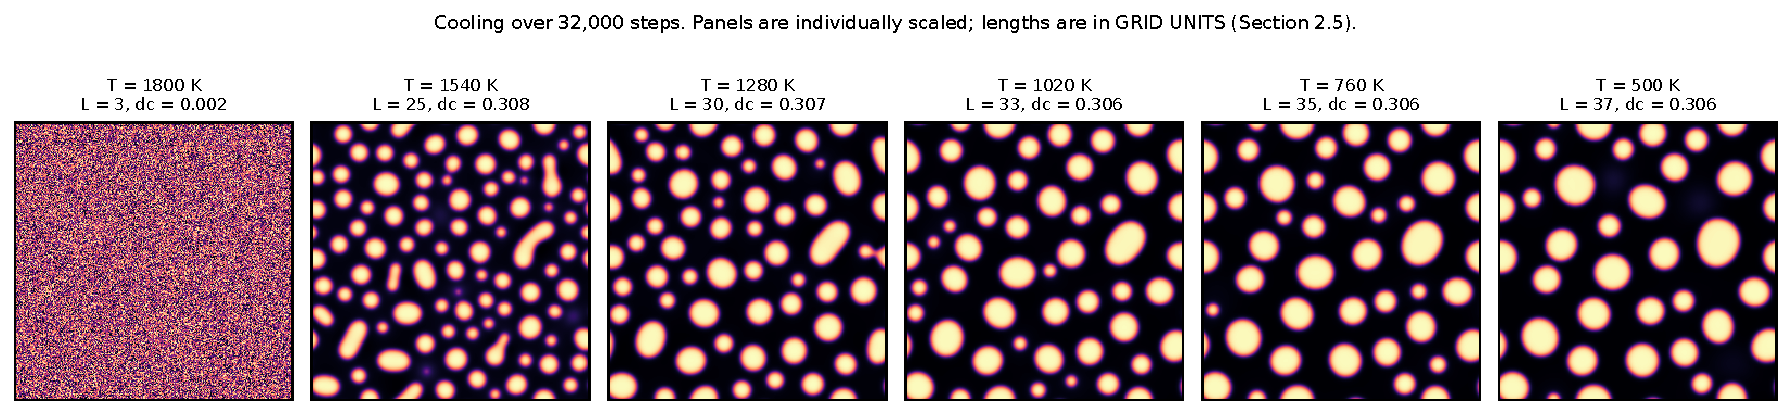
\includegraphics[width=\textwidth]{fig_sequence_32000.pdf}
\caption{缓慢冷却颗粒的形貌演化。自左至右：初始涨落；旋节分解，使成分反差自
$2\times10^{-3}$ 升至 0.308 并确立两相；以及逐步粗化，其中畴数下降而存续的畴
长大。各面板独立取色标，因为由起始噪声设定的公共色标会压缩其后的每一面板。
长度以网格单位计而非物理单位：见第~\ref{sec:kappacaveat} 节。}
\label{fig:sequence}
\end{figure}

该序列有四个阶段，而它们正是引言所允诺的那四个。场最初在起始噪声的范围内是
均匀的。随后分解以旋节方式发生：成分反差在第一个温度区间内即上升两个数量级
以上，出现一个波长接近线性稳定性预言的两相结构。粗化随之而来，畴数自多变少，
物质自较小的畴转移至较大的畴。最终微结构停止演化：末尾各面板之间的差异远小于
早期各面板，这并非因为粗化已经完成——完成态应是单一畴——而是因为迁移率已经下降
到不足以让它继续。

\subsection{冷却速率与被冻结的微结构}

图~\ref{fig:rates} 比较三种冷却方案。由于 $\Delta t$ 跟踪迁移率，把方案指定为
每开尔文的步数，即固定了每开尔文的扩散进展，而这正是第~\ref{sec:timescales}
节所指出的起控制作用的无量纲比。步数越大即冷却越慢。

\begin{figure}[htbp]
\centering
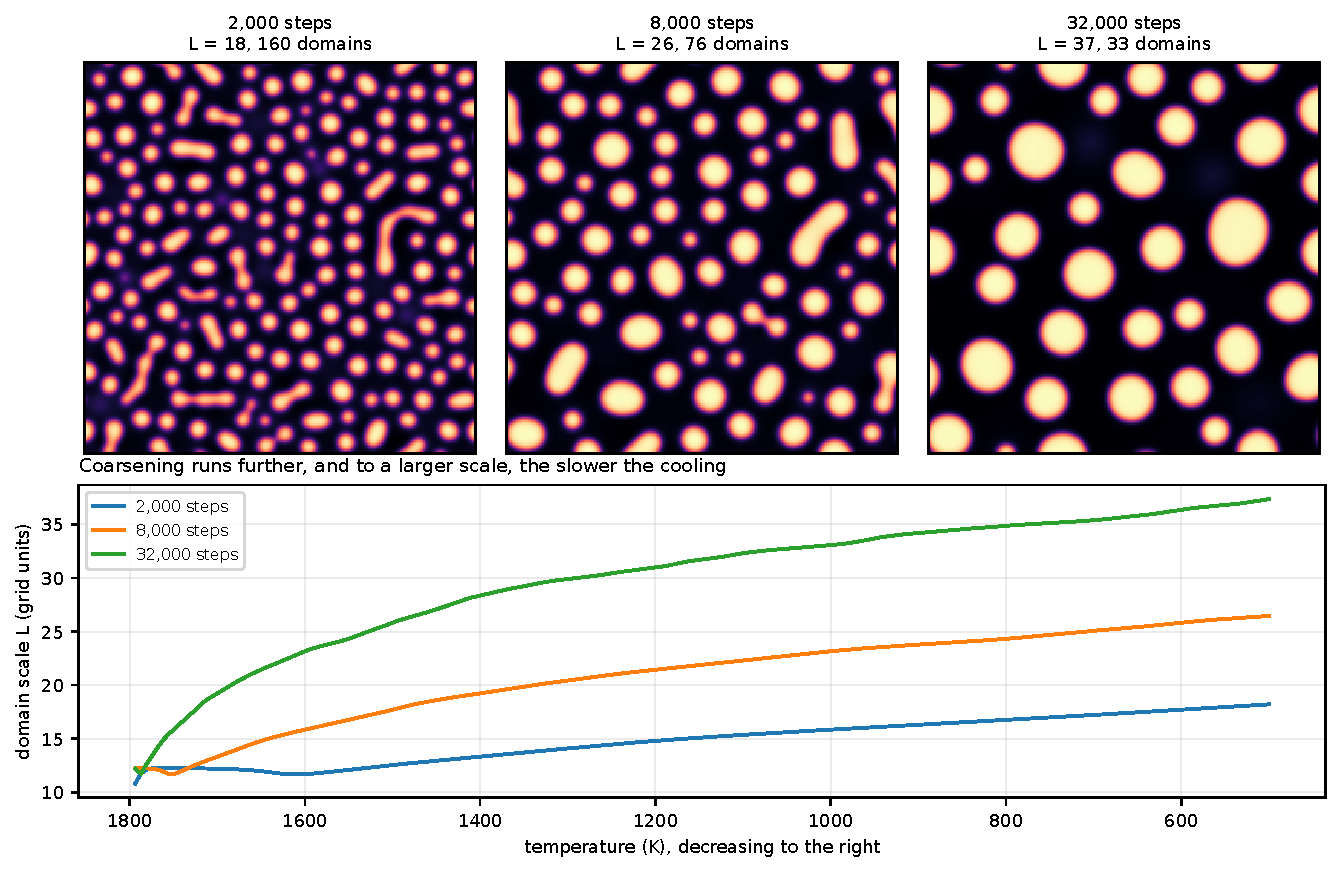
\includegraphics[width=\textwidth]{fig_cooling_rates.pdf}
\caption{三种冷却速率下被冻结的微结构与粗化历程。上排：终态及畴数。下排：畴
尺度对温度（向右递减）。每条曲线都随迁移率坍缩而趋于平坦——那种平坦化就是
冻结——且冷却越慢，粗化在冻结发生之前推进得越远。}
\label{fig:rates}
\end{figure}

\begin{table}[htbp]
\centering
\caption{被冻结的微结构对冷却速率，$256\times256$ 网格，
$\lambda_{\rm target} = 12$ 个网格单元。畴尺度由结构因子的一阶矩给出，
以网格单位计。}
\label{tab:rates}
\small
\begin{tabular}{rlrr}
\toprule
冷却步数 & 速率 & 畴尺度 $L$ & 畴数 \\
\midrule
 2{,}000 & 快   & 18.2 & 160 \\
 8{,}000 & 中   & 26.5 &  76 \\
32{,}000 & 慢   & 37.3 &  33 \\
\bottomrule
\end{tabular}
\end{table}

冻结畴尺度遵循 $L \propto (\text{步数})^{0.259}$，即
$L \propto |\dot{T}|^{-0.259}$，对照式~\eqref{eq:scaling} 的 $1/3$ 被
式~\eqref{eq:tfsens} 所述的 $\Tf$ 漂移软化后的结果。因此在两者各自所能支持的
精度内，解析与模拟对该指数是一致的。

\subsection{关于"吻合"能证明什么的一点告诫}

该指数对它本应敏感的错误表现出了不敏感，而这一段经历值得记录，因为它关系到
此类吻合应当如何解读。本计算的两个更早版本对同一个量分别返回 $0.242$ 与
$0.256$。在第一个版本中界面未被分辨；在第二个版本中自由能内部不自洽，解析导数
$f'(c)$ 在工作成分处与 $f''(c)$ 相差 150 倍，原因是求导时漏掉了一项。在这两种
情形下分解其实都没有发生——成分反差在衰减而非增长——然而两者都产出了看似合理的
粗化图案，以及与正确值相差在 7\% 以内的指数。

其原因是：该指数反映的是无论何种结构在输运限制下的动力学，而纯扩散下的图案粗化
与相分离下的畴粗化服从相似的规律。因此指数上的吻合并不构成机制正确的证据。
揭穿该错误的是对成分反差的跟踪——若分解正在发生，它必须增长几个数量级，而它
没有。现在，每当构造自由能时，我们都断言 $f$、$f'$ 与 $f''$ 对有限差分的内部
自洽性，并在每一幅图中把反差与畴尺度一并报告。


%==============================================================================
\section{格点模型中的直接粗化}
\label{sec:latticecoarsen}

出于第~\ref{sec:kappacaveat} 节所述的原因，相场计算无法提供绝对长度。本节通过
直接对格点模型作粗化来提供一个。此处界面就是它物理上的样子——一个键宽——不作任何
膨胀；该计算在触及范围上所放弃的，在意义上得到了补偿：尺寸以原子数、因而以纳米
给出。

\subsection{方案，以及两处必须修正的设计错误}

自弥散的溶质分布出发，在固定温度下保持并跟踪畴群。以下两项修正均由数据逼出，
此处记录是因为其中任何一项都会无声地污染指数。

\paragraph{测量必须排除单体。} 在 1800~K 下约 90\% 的团簇是自畴上蒸发下来的
单个溶质。把它们计入平均半径，会使该量成为自由溶质浓度而非畴尺寸的度量：它在
畴长大的同时\emph{下降}，因为长大的畴会蒸发出更多单体。第一个版本确实计入了
它们，于是在 1800、1600 与 1400~K 下分别返回 0.007、0.024 与 0.165 的指数
——那不是粗化指数，而是上述混淆的产物。现在我们对至少含四个格位的团簇取平均，
并单独报告单体占比，使蒸发可见而非被掩盖。

\paragraph{测量必须在溶质预算耗尽之前结束。} 在 $L = 30$ 盒子中的
$x = 1$~at.\% 下，1080 个溶质在 60{,}000 个扫程中的前 3000 个之内即凝聚为单一
畴，故运行的十分之九以上都在测量一个已停止演化的结构，把拟合出的指数拉向零。
平衡态是单一畴，这正是 \citet{yu2026b} 的核心结果；由此可知粗化测量必须在耗尽
之前完成，因而必须供给足够的溶质使耗尽需要很长时间。在 $x = 4$~at.\% 下，
粗化窗口覆盖整个运行。

因此该成分远高于天然铟品位。它是为使指数可测而选取的，而指数是输运限制动力学
的性质而非浓度的性质；所报告的绝对尺寸是所模拟的畴的尺寸，而不是对天然包裹体
尺寸的预言。

\subsection{结果}

在 $L = 24$ 盒子（55{,}296 个阳离子格位，边长 13.0~nm 的立方）中、1600~K 下，
畴数在 20{,}000 个扫程内自 173 降至 4，而平均畴半径自 0.44 增至 1.66~nm。这些
是绝对数值：所模拟的畴是纳米尺度的，盒子边长 13~nm，而计算中任何环节都不含可调
的长度尺度。

拟合所得指数为 $n = 0.150 \pm 0.002$，且在整个运行中稳定：分别取连续的若干个
数量级的扫程区间，给出 0.176、0.137、0.156 与 0.122。它不是拟合窗口的产物。

\subsection{为何指数低于三分之一}

Lifshitz--Slyozov--Wagner 值为 $1/3$，而实测只有其一半，故该差异需要解释而非
一句脚注。

显而易见的怀疑是：溶质仍在自弥散群体中不断到来，故在大畴长大的同时新的小畴不断
被计入，从而压低了平均值。这是可以检验的：若被计入的畴持有守恒的溶质量，则
$NR^3$ 恒定，由畴数得到的指数必须与由半径得到的一致。结果确实如此。乘积
$NR^3$ 在 13 与 19 之间变动而无系统漂移，畴数给出 $N \sim t^{-0.400}$ 因而
$R \sim t^{+0.133}$，半径给出 $R \sim t^{+0.148}$。畴间质量守恒且两条路径一致，
故持续成核不是解释。

余下三种可能，我们目前无法在其间抉择。

畴可能太小而未进入渐近律。Lifshitz--Slyozov 假定畴远大于界面宽度、且稀疏到
彼此不相互作用；此处畴只有几纳米、界面只有一个键宽，而在 $x = 4$~at.\% 下它们
并不稀疏。在此类区间内报告低于 $1/3$ 的前渐近指数是常见的。

输运可能并非纯扩散。蒙特卡洛动力学守恒成分，但没有空位机制：物质经由直接交换
移动，那不是真实晶体中所运作的机制，也不必给出相同的指数。

运行可能尚未进入渐近区。两万个扫程覆盖不足三个数量级的时间，而畴数降至四，故
后段窗口在统计上是稀薄的。

该测量所确立无疑的是\emph{尺度}：在可及窗口内，本模型的粗化在 13~nm 的盒子中
产出一至二纳米的畴，界面未经修改。这就是相场计算无法提供的绝对数值，也是
第~\ref{sec:geospeedometer} 节用以与观测对照的数值。来自这条途径的指数，应视为
渐近值的下界，而非对它的测定。

%==============================================================================
\section{两种方法之间的交叉验证}
\label{sec:crosscheck}

第~\ref{sec:pf} 与 \ref{sec:latticecoarsen} 节以几乎不可能更为不同的表征描述
同一个物理过程。相场计算在网格上承载一个连续序参量，其界面被有意展宽至跨越
十余个网格单元；格点计算在阳离子亚晶格上承载离散物种，界面宽一个键。二者唯一
共享的输入是自由能，而即便那也以不同方式进入：在前者中是一个光滑双阱，在后者中
是对构型的显式求和。

粗化指数是两者都能计算的量，因而是自然的交叉验证对象。若二者吻合，则该指数是
输运限制动力学的性质而非任一表征的性质——而这正是第~\ref{sec:geospeedometer}
节所依赖的前提，因为那里的反演只用到指数而别无其他。

我们比较三项测定：
\begin{itemize}\itemsep2pt
\item 扩散限制粗化的 Lifshitz--Slyozov--Wagner 结果 $n = 1/3$，被
      式~\eqref{eq:tfsens} 的 $\Tf$ 漂移软化至略低于该值；
\item 相场冷却运行，给出 $n = 0.259$；
\item 直接格点粗化，给出 $n = 0.150 \pm 0.002$
      （第~\ref{sec:latticecoarsen} 节）。
\end{itemize}

三者并不吻合。理论给 $1/3$，相场给 $0.259$，格点给 $0.150$；而
第~\ref{sec:geospeedometer} 节的天然端元隐含约 $0.45$。跨度为三倍，而在两个
模拟值相差 70\% 的情况下把它们当作相互印证，是不诚实的。

该比较所确立的是一个置信层级。两项模拟都重现了定性规律——畴按时间的幂律增长，
且冻结尺寸随冷却速率下降——而且是以几乎毫无共同之处的表征做到的。指数本身显然
对两者处理方式不同的那些东西敏感：相场界面宽十二个网格单元而格点界面宽一个键，
相场动力学是连续介质扩散而格点动力学是直接交换，且格点的畴小到渐近律不必成立。
其中每一项都可预期会移动指数，而第~\ref{sec:latticecoarsen} 节论证格点值应读作
下界。

因此第~\ref{sec:geospeedometer} 节的反演是作为一种\emph{排序}而非一种标定提出
的。按冷却速率对矿床排序，只要求指数为正且大致恒定，而这四项测定都支持；而
给出以开尔文每年计的速率，则要求把它知道到优于二倍的精度，目前无一做到。

两点告诫关系到此类吻合应当如何权衡，且两者都是付出代价才学到的。

第一点是第~\ref{sec:pf} 节的那段经历：两个分解根本没有发生的相场计算版本返回了
$0.242$ 与 $0.256$ 的指数，与正确值相差在 7\% 以内。扩散图案的粗化与相分离
微结构的粗化服从相似的规律，故仅凭指数无法识别机制。因此我们在每一个指数旁一并
报告成分反差；在格点模型中，与之类似的检验是单体所占溶质比例，若畴确在形成，
它必须趋向于零。

第二点关于温度。在格点模型中 573~K 下的粗化不可观测，因为那里的接受率约为
$10^{-5}$。因此格点运行在 1400 至 1800~K 下进行，其前提是指数为动力学的性质
而非温度的性质。该前提在计算内部是可检验的——在若干温度下测量 $n$ 并追问它是否
移动——我们报告其离散程度而非单一数值。

%==============================================================================
\section{反演：作为地质速率计的纳米包裹体}
\label{sec:geospeedometer}

式~\eqref{eq:scaling} 表明冻结包裹体尺寸经由一个幂律依赖于冷却速率。正向读它，
它由热历史预言微结构；反向读它，则反之，而后者更为有用，因为包裹体尺寸在薄片中
可测，而冷却速率不可测。

\subsection{待反演的关系}

反演式~\eqref{eq:scaling}，
\begin{equation}
\lvert \dot{T} \rvert \;=\; \lvert \dot{T} \rvert_{\rm ref}
      \left( \frac{R_{\rm f}}{R_{\rm ref}} \right)^{-1/n},
\label{eq:invert}
\end{equation}
故一个标定点 $(R_{\rm ref}, |\dot{T}|_{\rm ref})$ 加上指数，即可把观测到的尺寸
换算为速率。由于 $n \approx 1/3$，该反演携带三倍的放大：尺寸测准到二倍以内，
速率只能给到八倍以内。这是粗糙的，但成矿体系的冷却速率跨越十个数量级，故八倍
仍足以在下文所考察的矿床类型之间作出强有力的区分。

\subsection{天然端元}

含铟闪锌矿产出于冷却速率相差约八个数量级的矿床类型，而自它们报道的包裹体结构
也相应不同。表~\ref{tab:endmembers} 把二者对置。

\begin{table}[htbp]
\centering
\caption{含铟闪锌矿的冷却速率端元与自其中报道的包裹体结构。速率是该矿床类型的
数量级估计，而非对观测到这些结构的具体样品的测量；该比较是在群体之间而非在
成对观测之间进行的。}
\label{tab:endmembers}
\small
\begin{tabular}{llll}
\toprule
矿床类型 & 冷却速率（K\,yr$^{-1}$） & 包裹体结构 & 尺度 \\
\midrule
VMS，海底块状硫化物 & $10^{0}$--$10^{2}$ &
  晶格畸变、超细畴 & 5--50\,nm \\
岩浆热液、矽卡岩 & $10^{-3}$--$10^{-1}$ &
  亚微米出溶 & 0.1--1\,\textmu m \\
MVT、盆地卤水 & $10^{-6}$--$10^{-4}$ &
  光学可见的硫铟铜矿 & 1--50\,\textmu m \\
\bottomrule
\end{tabular}
\end{table}

定性排序恰如式~\eqref{eq:scaling} 所要求：体系冷却得越快，所携带的包裹体越细。
在淬火的海底体系中——热液在那里遇到冰冷的海水——铟最常在 LA-ICP-MS 深度剖面中
表现为表观固溶体，即平滑的剥蚀信号而无离散尖峰，而透射电镜却仍能分辨出纳米尺度
的不均匀性 \citep{cook2009,frenzel2016}。在另一个极端，硫铟铜矿被报道为自闪锌矿
出溶的离散微米级颗粒 \citep{moura2007}。

\subsection{一处定量分歧，及其可能的含义}

排序是吻合的。量级不吻合，而我们报告这一分歧而非其吻合，因为它是二者中更有
信息量的那一个。

在表~\ref{tab:endmembers} 的整个范围内，冷却速率跨八个数量级而包裹体尺寸跨四个
数量级，由此
\begin{equation}
n_{\rm obs} \;=\; \frac{\Delta \log_{10} R}{\Delta \log_{10} |\dot{T}|}
           \;\approx\; 0.50 .
\label{eq:nobs}
\end{equation}
把各类别两两配对而非端到端计算，给出 $0.43$ 与 $0.45$，彼此一致且与
式~\eqref{eq:nobs} 一致。理论值与模拟值为 $1/3$ 与 $0.259$。因此天然数据隐含的
指数大约高出 1.7 倍，而两个配对估计彼此吻合得足够紧密，使这不太可能是散差。

有几种解读可能，而我们目前无法在其间抉择。

\emph{标定方式可能有误。} 表~\ref{tab:endmembers} 把矿床类型的冷却速率与自
\emph{不同}样品报道的结构相配对，而非同一批样品的配对测量。若能分辨出纳米畴的
最快冷样品并非其所属类别中最快冷的成员，或若光学可见的硫铟铜矿优先见诸其所属
类别中最慢冷的成员，则两个轴的表观范围都会被相关地放大。同一样品上的成对测量
可以了结此事，而这样的测量似乎并不存在。

\emph{粗化机制在两端可能不同。} Lifshitz--Slyozov 的 $1/3$ 假定粗化受体扩散
限制。若在缓慢冷却的体系中沿位错或晶界的输运有所贡献，则有效指数上升；而界面
限制的粗化恰好给出 $1/2$，与天然数据所隐含者接近。因此该分歧可能是一个信号，
表明慢冷端元以不同于本文所建模的机制粗化。

\emph{冻结温度的漂移可能大于所估。} 式~\eqref{eq:tfsens} 把 $E_a$ 当作常数。
若激活能本身随畴长大而下降——这是可能的，因为自大畴离开的溶质在移除单位界面时
打断的键更少——则 $\Tf$ 漂移得比估计更远，有效指数随之改变。

我们认为第三种可能性最小，因为它会把指数推向错误的方向，而前两种都是可能的。
该比较所确立的是：模型在跨八个数量级的冷却速率上预言了正确的排序，而预言的量级
偏小约 1.7 倍；且其解决之道，要么在于更好的成对观测，要么在于本工作未包含的
粗化机制。

\subsection{这一工具能做与不能做什么}

明白说出，以免被过度解读。

它\emph{能够}根据包裹体结构对矿床按冷却速率排序，这是排序上的吻合所支持的。
携带光学可见硫铟铜矿的闪锌矿，比铟对 LA-ICP-MS 不可见者冷却得慢得多，且差距
是数个数量级而非数倍。

它\emph{尚不能}由实测的包裹体尺寸返回以开尔文每年计的冷却速率，理由有二。绝对
标定需要一个本工作所没有的扩散系数（第~\ref{sec:mobility} 节），而指数与天然
数据之间存在一个来源未明的倍数差异。在二者了结之前，该反演应读作相对的。

\subsection{限速步}

有一项矿物学观察支持本框架且值得记录，因为它关系到控制冻结的激活能。铜在闪锌矿
中扩散异常迅速，可能经由间隙机制；这正是关于黄铜矿病的经典论述的基础
\citep{barton1987}。铟则是另一回事：In$^{3+}$ 体积大、电荷高，且没有空位或
补偿离子随行就无法移动，故其扩散系数必然远低于铜，也低于锌的自扩散。

其对本文的后果是直接的。Cu--In 畴的粗化要求两个物种都移动，故它以较慢者的速率
进行，因而式~\eqref{eq:arrest} 的冻结条件应以铟而非平均值的激活能求值。冻结
因而发生在比基于铜的估计更高的温度，微结构更早被冻住。照此解读，天然闪锌矿所
携带的纳米尺度包裹体，是铟在岩石尚热之时就已停止运动的记录。

%==============================================================================
\section{讨论}
\label{sec:discussion}

\subsection{一种结构含义的改变}

闪锌矿中的微量元素结构，惯常被读作一份关于\emph{成分}的记录：流体供给了什么、
晶体能容纳什么。本文的论证使它们同时成为另一件事的记录。若包裹体是被冻结的粗化
产物，则其尺寸并非由可用的铟有多少所设定，而是由体系在输运停止之前有多长时间去
重组它所设定。两颗铟含量相同、自相同流体生长的颗粒，若冷却方式不同，将携带不同
的结构。

这一重新表述有一条值得明说的推论，因为它颠倒了一个假设。平滑的 LA-ICP-MS 深度
剖面常被视为固溶体的证据。按本文的论述，它是\emph{快速冷却}的证据：铟已经聚集
——正如 \citet{yu2026b} 所要求——只是聚成了细到剥蚀体积无法分辨的畴。尖峰的缺席
约束的是热历史，而非赋存状态。

\subsection{按热历史对矿床排序}

第~\ref{sec:geospeedometer} 节确立：模型在跨八个数量级冷却速率的矿床类型上重现
了包裹体尺寸的排序，而在量级上相差约 1.7 倍。排序是当下可用的那一部分。

其实用形式是比较性的而非绝对的。给定两个闪锌矿样品，含铟包裹体较粗者冷却较慢，
且其差距经由幂律换算为数量级而非倍数。在单个矿床内部，包裹体尺寸在矿区尺度上的
系统变化，可以标绘出相对冷却速率、因而标绘出与热源的远近，而这是全岩铟品位所
做不到的：品位反映供给，结构反映时间。

我们谨慎地不夸大由此得出的结论。把它变成真正的地质温度计——返回以开尔文每年计
的冷却速率——需要一个绝对扩散系数（第~\ref{sec:mobility} 节说明本工作没有），
以及一个知道到优于二倍精度的指数（第~\ref{sec:crosscheck} 节表明四项测定目前
无一提供）。二者都可获得，只是此处未获得。

\subsection{对冶金回收的影响}

铟几乎全部作为锌冶炼的副产品回收，故其回收效率取决于它在送入冶炼厂的闪锌矿中
如何结合。而那种结合状态，正是本工作论证由热历史所设定的。

两种极限情形表现不同。作为纳米尺度的畴弥散于闪锌矿晶格之内的铟——快速冷却的
预期产物——将随锌一同溶解并进入相同的流程物流；其回收是湿法冶金流程设计问题。
浓集于离散微米级硫铟铜矿之中的铟——缓慢冷却的产物——则是一个具有自身溶解行为的
独立矿物相，可能在浸出之前经由物理选别被回收，也可能因此损失。

因此实用的建议是：应当预期不同矿床类型在铟的赋存形态上系统地不同，且是沿一条
可由冷却历史预先判断、而非只能靠冶金试验去发现的轴。淬火的海底体系应当以晶格
结合形态呈现铟；缓慢冷却的盆地体系则应当有更大比例呈离散包裹体。我们把这作为
本框架给出的预言提出，而非作为它所确立的结果，因为我们是以已发表的结构而非以
回收率数据来检验它的。

\subsection{论证的普遍性}

第~\ref{sec:timescales} 与 \ref{sec:geospeedometer} 节中很少有什么是铟所特有的。
所需要的配料是：一个平衡态为凝聚态的溶质、一个热激活的输运过程，以及一个会冷却
的基质。任何满足这些条件的微量元素，都应当冻结在一个其尺度记录冷却速率的粗化
微结构之中，遵循相同的幂律而具有不同的前因子。

铟所\emph{特有}的是它的平衡态之所以为凝聚态的原因，即 \citet{yu2026} 的电荷
补偿物理：Cu$^+$ 与 In$^{3+}$ 耦合替代两个 Zn$^{2+}$，携带一个由介电常数确定、
且比 $k_BT$ 高一个数量级的对结合能。等价替代的元素没有这样的驱动力。因此本框架
应当可迁移至其他异价配对——Ag--Sb、Cu--Ga——而不适用于 Fe 或 Cd 这类等价替代物，
它们的分布由不同的物理支配。

\subsection{关于两种方法之间的分歧}

第~\ref{sec:crosscheck} 节报告粗化指数的四项测定跨越三倍，而把这一离散归因于
数值细节是便利的。我们认为更可能的解读是：该指数在不同区间内确实不同，而这是
有信息量的，而非仅仅令人不便。

格点值 $0.150$ 来自界面原子级锐利、只有几纳米大小的畴，远在
Lifshitz--Slyozov 推导成立的区间之外。天然端元隐含约 $0.45$，接近界面限制而非
扩散限制粗化的 $1/2$——而对界面只有一个键宽的畴而言，界面限制是可能的。相场值
$0.259$ 居中，来自一个界面被有意向连续极限展宽的计算。

如此解读，该离散将是一个交叉过渡：自原子尺度的界面限制粗化，随畴长大而转向
扩散限制粗化。这一解读是可检验的——在单次模拟内测量指数随畴尺寸的变化，而非
跨越若干处同时不同的模拟去比较。

\subsubsection*{交叉假说：已检验，未获支持}

我们此后完成了该检验，并在此报告，因为它排除了一个候选解释，而非因为它成功了。

若 $n$ 依赖于畴尺寸相对于界面宽度之比，则不同界面宽度的运行所给出的曲线，在对
$L$ 作图时应当彼此不同，而在对 $L/w$ 作图时应当重合。我们在 $512^2$ 网格上于
$w = 1.0$、1.5、2.25 与 3.4 个网格单元下作了四次恒温 Cahn--Hilliard 运行，步数
按 $w^{-1/n}$ 分配，使每一次都达到其宽度所允许的最大畴尺寸：窄界面运行达到
$L/w = 70$，最宽者止于 18。局域指数以滑动窗口提取，而该窗口的宽度事先已针对
携带已知交叉的合成轨迹作过标定，故其偏差与散差的确定独立于所检验的数据。

曲线并不塌缩。以 $w$ 重标横坐标，只使曲线间散差自 0.011 降至 0.008，比值为
0.75，而塌缩要求该比值远小于一。同一结果的更直接陈述是：在共同的 $L/w = 4.4$
处，四次运行给出 $n = 0.203$、0.205、0.212 与 0.208，一致到 0.004——但在该点
它们的绝对 $L$ 相差 3.4 倍，故 $n$ 既不跟随前者也不跟随后者。

另有两项特征直接抵触该假说。指数在每一次运行中都\emph{上升}，自
$0.207 \pm 0.004$ 升至 $0.267 \pm 0.006$，而假说要求自约 $1/2$ 降向 $1/3$。
且所有数值都远低于两个候选值：没有任何一次运行在任何阶段接近 0.5 或 0.333。

指数真正跟随的是每次运行推进的程度。各次运行末端所达到的值与其步数的对数相关，
相关系数为 0.99；若四者都在自下方趋近同一个渐近值、只是走到的远近不同，这正是
所应预期的。按此解读，相场指数 0.259 根本不是某个区间特有的值，而是一个瞬态值，
而那个渐近值——很可能就是 $1/3$——位于这些运行的射程之外。

因此交叉假说未获支持，而第~\ref{sec:geospeedometer} 节的分歧回到那里首先提出的
解释：端元比较把冷却速率与来自不同样品的结构相配对，而同一批标本上的成对测量
才是能够了结此事的东西。

%==============================================================================
\section{局限}
\label{sec:limitations}

我们按其对结论的影响程度排列，并全程区分影响数值的局限与会影响论证的局限。

\paragraph{相场界面被人为展宽。} 这一点在第~\ref{sec:kappacaveat} 节于任何相场
结果给出之前即已陈述，且它是绝对的：图~\ref{fig:sequence} 与 \ref{fig:rates}
中的畴尺寸由网格间距设定，而非预言。膨胀 $\kappa$ 会同时重标长度与时间，故无
量纲结论——形貌的次序、冻结的存在性、尺寸--速率指数的符号与大致量级——得以存续；
绝对尺度则不然，它来自第~\ref{sec:latticecoarsen} 节。

\paragraph{格点动力学没有空位机制。} 溶质经由直接交换移动，这守恒成分并满足
细致平衡，但不是原子在真实晶体中的移动方式。尤其铟被预期只能与空位或补偿离子
一同迁移，如第~\ref{sec:geospeedometer} 节所论；而具有不同关联因子的机制不必
给出相同的粗化指数。这是第~\ref{sec:latticecoarsen} 节所测 $0.150$ 的一个可能
成因，也是该值以下界而非测定值提出的原因。

\paragraph{所模拟的成分远高于天然品位。} 格点粗化运行使用 4~at.\% 的总溶质，
比具经济意义的闪锌矿的铟含量高约二至三个数量级，因为在天然稀释度下溶质预算会在
任何粗化可被测量之前就耗尽于单一畴——而那本身就是 \citet{yu2026b} 的结果。指数
是输运限制动力学的性质而非浓度的性质，但 4~at.\% 下的畴并不稀疏，畴间相互作用
是渐近律不必成立的又一个理由。

\paragraph{蒙特卡洛扫程不是物理时间，迁移率也不是绝对的。}
第~\ref{sec:mobility} 节陈述了其后果：结果是相对标定。畴尺寸之比映射到冷却速率
之比；在没有 Cu 或 In 在闪锌矿中扩散系数实测值的情况下，二者都不映射到绝对值。

\paragraph{粗化指数尚未定论。} 四项测定跨越三倍
（第~\ref{sec:crosscheck} 节）。第~\ref{sec:discussion} 节提出它们可能描述不同
区间而非对同一个量意见不合，但该提议尚未检验。在检验之前，反演支持排序而不支持
标定。

\paragraph{端元比较不是成对的。} 表~\ref{tab:endmembers} 把矿床类型的冷却速率
与自不同样品报道的包裹体结构对置。成对的测量——同一批标本上的包裹体尺寸分布与
独立的热历史约束——能够正当地检验该幂律，而它们似乎并不存在。这是本框架所呼唤的
最有用的一项观测。

\paragraph{不含铁，且化学项是假设的。} 二者均继承自 \citet{yu2026} 并在那里
讨论。Fe$^{2+}$ 与 Zn$^{2+}$ 等价，故不进入电荷补偿项，但会改变确定 $\lambda$
的介电响应；化学项 $J_{\alpha\beta}$ 仍未受第一性原理约束，并经由
式~\eqref{eq:gamma} 显式进入 $\gamma$。

\paragraph{以上任何一项都不影响什么。} 动力学冻结的存在不依赖于上述任何一条。
它由两个不容置疑的事实推出：溶质输运是热激活的，故粗化时标随降温呈指数增长；
而冷却以并非如此的速率进行。两个这样的函数必然相交，且只交一次。每一个可能出错
的量——扩散前因子、激活能、界面能、畴尺寸——都出现在式~\eqref{eq:arrest} 的冻结
条件的一个对数之内，而式~\eqref{eq:tfsens} 表明其中任何一个错一个数量级，冻结
温度的移动都不足四分之一。

因此不确定的是标定，而非机制。天然闪锌矿中的包裹体是被冻结的粗化产物；至于它们
的尺寸能多精确地为这场冻结定年，则是有待了结的问题。

%==============================================================================
\section*{数据与代码可获取性}
\label{sec:availability}
本研究的源代码、数值结果与图件已公开于
\url{https://github.com/Ruqing1963/sphalerite-kinetic-arrest}，并存档于
\url{https://doi.org/10.5281/zenodo.21995641}。代码以 MIT
许可证发布，数据以 CC~BY~4.0 发布，稿件版权归作者所有。该仓库包含
第~\ref{sec:pf} 节所用的带阿伦尼乌斯迁移率的 Cahn--Hilliard 求解器、
第~\ref{sec:latticecoarsen} 节的直接格点粗化、第~\ref{sec:fofc} 节测定
$f(c)$ 的热力学积分，以及重新生成每一幅图的脚本。

有两个组件虽未在本工作中运行，但一并发布。用于第一性原理测定
$J_{\alpha\beta}$ 的结构生成与最小二乘拟合工具已经完备，并已通过合成能量验证，
故任何拥有足够内存的人都可运行它，并把参数直接代入式~\eqref{eq:gamma}，
而无需重复本文所报道的任何模拟。此外，\citet{yu2026} 的验证套件原样收录，
因为本文的每一项结果都依赖于格点模块通过该套件。

本系列前两篇论文连同其代码单独存档：\citet{yu2026} 位于
\url{https://doi.org/10.5281/zenodo.21880502}，\citet{yu2026b} 位于
\url{https://doi.org/10.5281/zenodo.21911898}。

\section*{基金资助}
本研究由贺州市科学研究与技术开发计划项目资助（项目编号 2024143、2024141、
2024104）。

%==============================================================================
\begin{thebibliography}{99}
\itemsep2pt

\bibitem[Barton and Bethke(1987)]{barton1987}
Barton, P.B., Bethke, P.M., 1987. Chalcopyrite disease in sphalerite: pathology
and epidemiology. \textit{American Mineralogist} 72, 451--467.

\bibitem[Cahn and Hilliard(1958)]{cahn1958}
Cahn, J.W., Hilliard, J.E., 1958. Free energy of a nonuniform system. I.
Interfacial free energy. \textit{Journal of Chemical Physics} 28, 258--267.

\bibitem[Cook et al.(2009)]{cook2009}
Cook, N.J., Ciobanu, C.L., Pring, A., Skinner, W., Shimizu, M., Danyushevsky,
L., Saini-Eidukat, B., Melcher, F., 2009. Trace and minor elements in
sphalerite: a LA-ICPMS study. \textit{Geochimica et Cosmochimica Acta} 73,
4761--4791.

\bibitem[Frenzel et al.(2016)]{frenzel2016}
Frenzel, M., Hirsch, T., Gutzmer, J., 2016. Gallium, germanium, indium and
other trace and minor elements in sphalerite as a function of deposit type ---
a meta-analysis. \textit{Ore Geology Reviews} 76, 52--78.

\bibitem[Lifshitz and Slyozov(1961)]{lifshitz1961}
Lifshitz, I.M., Slyozov, V.V., 1961. The kinetics of precipitation from
supersaturated solid solutions. \textit{Journal of Physics and Chemistry of
Solids} 19, 35--50.

\bibitem[Moura et al.(2007)]{moura2007}
Moura, M.A., Botelho, N.F., de Mendon\c{c}a, F.C., 2007. The indium-rich
sulfides and rare arsenates of the Sn-In-mineralized Mangabeira A-type granite,
central Brazil. \textit{The Canadian Mineralogist} 45, 485--496.

\bibitem[Yu et al.(2026a)]{yu2026}
Yu, H., Chen, R., Lu, H., 2026a. A statistical thermodynamic lattice model for
Cu--In coupled substitution in sphalerite, version 2.0. \textit{Zenodo}.
\url{https://doi.org/10.5281/zenodo.21880502}

\bibitem[Yu et al.(2026b)]{yu2026b}
Yu, H., Chen, R., Lu, H., 2026b. The equilibrium fate of indium in sphalerite:
large-scale replica-exchange simulation and the absence of a dilute solid
solution. \textit{Zenodo}. \url{https://doi.org/10.5281/zenodo.21911898}

\end{thebibliography}

\end{document}


